\newpage
\section{Конструкторская часть}

Рассмотрим сортировку пузырьком, шейкером и быструю сортировку.

\subsection{Функциональная модель}

На рисунке \ref{img:IDEF0} представлена функциональная модель IDEF0 уровня 1.

\begin{figure}[H]
    \centering
    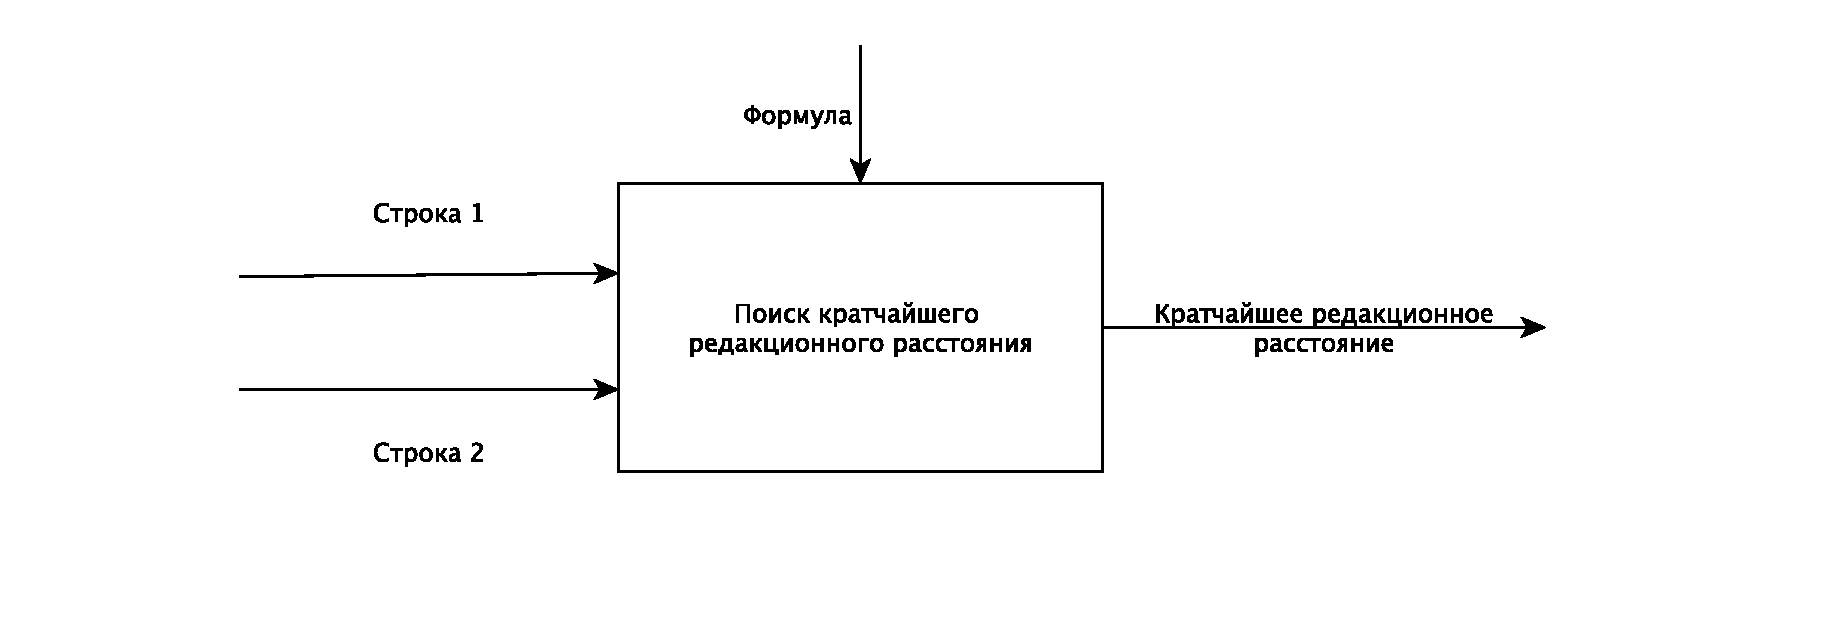
\includegraphics[scale=0.5]{IDEF0}
    \caption{Функциональная модель IDEF0 уровня 1}
    \label{img:IDEF0}
\end{figure}

\subsection{Схемы алгоритмов}

На рисунке \ref{img:bubble} изображена схема алгоритма сортировки пузырьком.

\begin{figure}[H]
    \centering
    \includegraphics[scale=0.55]{Bubble}
    \caption{Сортировка пузырьком}
    \label{img:bubble}
\end{figure}

На рисунке \ref{img:shaker} изображена схема алгоритма сортировки шейкером.

\begin{figure}[H]
    \centering
    \includegraphics[scale=0.8]{Shaker}
    \caption{Сортировка шейкером}
    \label{img:shaker}
\end{figure}

На рисунке \ref{img:qsort} изображена схема алгоритма быстрой сортировки.

\begin{figure}[H]
    \centering
    \includegraphics[scale=0.45]{QSort}
    \caption{Быстрая сортировка}
    \label{img:qsort}
\end{figure}

Произведем теоретическую оценку трудоемкости алгоритмов сортировки

\begin{enumerate}
    \item \textbf{Сортировка пузырьком}

        В лучшем случае, когда массив будет отсортирован, трудоемкость будет считать
        по формуле \ref{eq:bubble-good}.

        \begin{equation}\label{eq:bubble-good}
            f = 1 + 2N + \frac{N(N-1)}{2} \cdot 6 =
            3N^2 - N + 1
        \end{equation}

        В худшем случае, когда массив будет обратно отсортирован, трудоемкость будет
        считаться по формуле \ref{eq:bubble-bad}.

        \begin{equation}\label{eq:bubble-bad}
            f = 1 + 2N + \frac{N(N-1)}{2} \cdot 11 =
            \frac{11}{2}N^2 - \frac{7}{2}N + 1
        \end{equation}

        И в лучшем, и в худшем случае, сортировка пузьком имеет трудоемкость $O(N^2)$.

    \item \textbf{Сортировка шейкером} \cite{knuth}

        И в лучшем, и в худшем случае, сортировка шейкером иммет трудоемкость $O(N^2)$

    \item \textbf{Быстрая сортировка} \cite{knuth}

        В лучшем случае, когда массив упорядочен, трудоемкость равна $O(N \cdot \ln(N))$.

        В худшем случае, когда массив обратно упорядочен, трудоемкость равна $O(N^2)$.
\end{enumerate}

\subsection{Выводы}

Сортировка пузырьком и сортировка шейкером имеют одинаковую трудоемкость $O(N^2)$, но
по коэффициентам видно, что шейкерная сортировка быстрее пузырька в 4 раза. Быстрая
сортировка имеет трудоемкость $O(N \cdot \ln(N))$ из чего можно сделать вывод, что
быстрая сортировка на порядок быстрее двух других.
